\section{Running-Job Priority (HTCondor \texttt{JobPrio})}\label{ch:11}

\subsection{Problem statement}

Once clusters are submitted, they compete for OSG slots. The running-job priority steers already-submitted
clusters toward balanced running counts, computed by
\texttt{condor\_\allowbreak{}io/\allowbreak{}run\_\allowbreak{}priority\_\allowbreak{}map.\allowbreak{}py}.

\subsection{Scope boundary}

\textbf{This system writes only HTCondor \texttt{JobPrio}. It never writes
\texttt{submissions.\allowbreak{}priority}.} It has no effect on which waiting request is submitted next; it
only reorders work already in the local HTCondor queue.

\subsection{Cluster selection}

It queries the shared owner \texttt{gemc}'s live batches and selects the
\texttt{-\allowbreak{}-\allowbreak{}max-\allowbreak{}running} \textbf{oldest} clusters (production: 20), so the
balancing effort concentrates on the clusters closest to completion.

\subsection{Average-RUN balancing}

It computes the average running-job count over the selected clusters and maps each cluster to an integer
priority in \texttt{[-\allowbreak{}5, 5]} via
\texttt{\_\allowbreak{}priority\_\allowbreak{}from\_\allowbreak{}ratio(run, avg) =\allowbreak{}
clamp(round(5$\cdot$(1 $-\allowbreak{}$ run/\allowbreak{}avg)), $-\allowbreak{}$5, 5)}. Clusters below average
(fewer running jobs) get positive priority and run preferentially; clusters above average get negative
priority; exactly-average clusters get 0.

\subsection{Application to HTCondor}

With \texttt{-\allowbreak{}-\allowbreak{}apply}, the map is written to \texttt{JobPrio} for every job in each
selected cluster (target-0 and unselected clusters are left untouched). \texttt{-\allowbreak{}p} prints the old
and proposed values as a read-only preview.

\subsection{Per-cluster (not per-user) balancing}

Balancing is per cluster, not per portal user, precisely because every cluster shares the owner \texttt{gemc}
--- HTCondor cannot distinguish users, so the unit of balancing is the cluster.

\subsection{Preview vs. apply, and cadence}

\texttt{-\allowbreak{}p} previews, \texttt{-\allowbreak{}a} applies. Production runs every ten minutes:

\begin{lstlisting}
7-59/10 * * * * $sg/run_with_lock_and_log.zsh -l /home/gemc/logs \
    $sg/condor_io/run_priority_map.py -p -a -m 20
\end{lstlisting}

\subsection{Independence of the two priority systems}

The pending-queue calculator (Chapter 10) and this runtime balancer are independent: they read overlapping
inputs (live running counts) but write different stores toward different goals, and neither value is inferred
from the other. Conflating them is the single most common misunderstanding of the system; the code, the README,
and this note keep them strictly separate.

\begin{figure}[htbp]
  \centering
  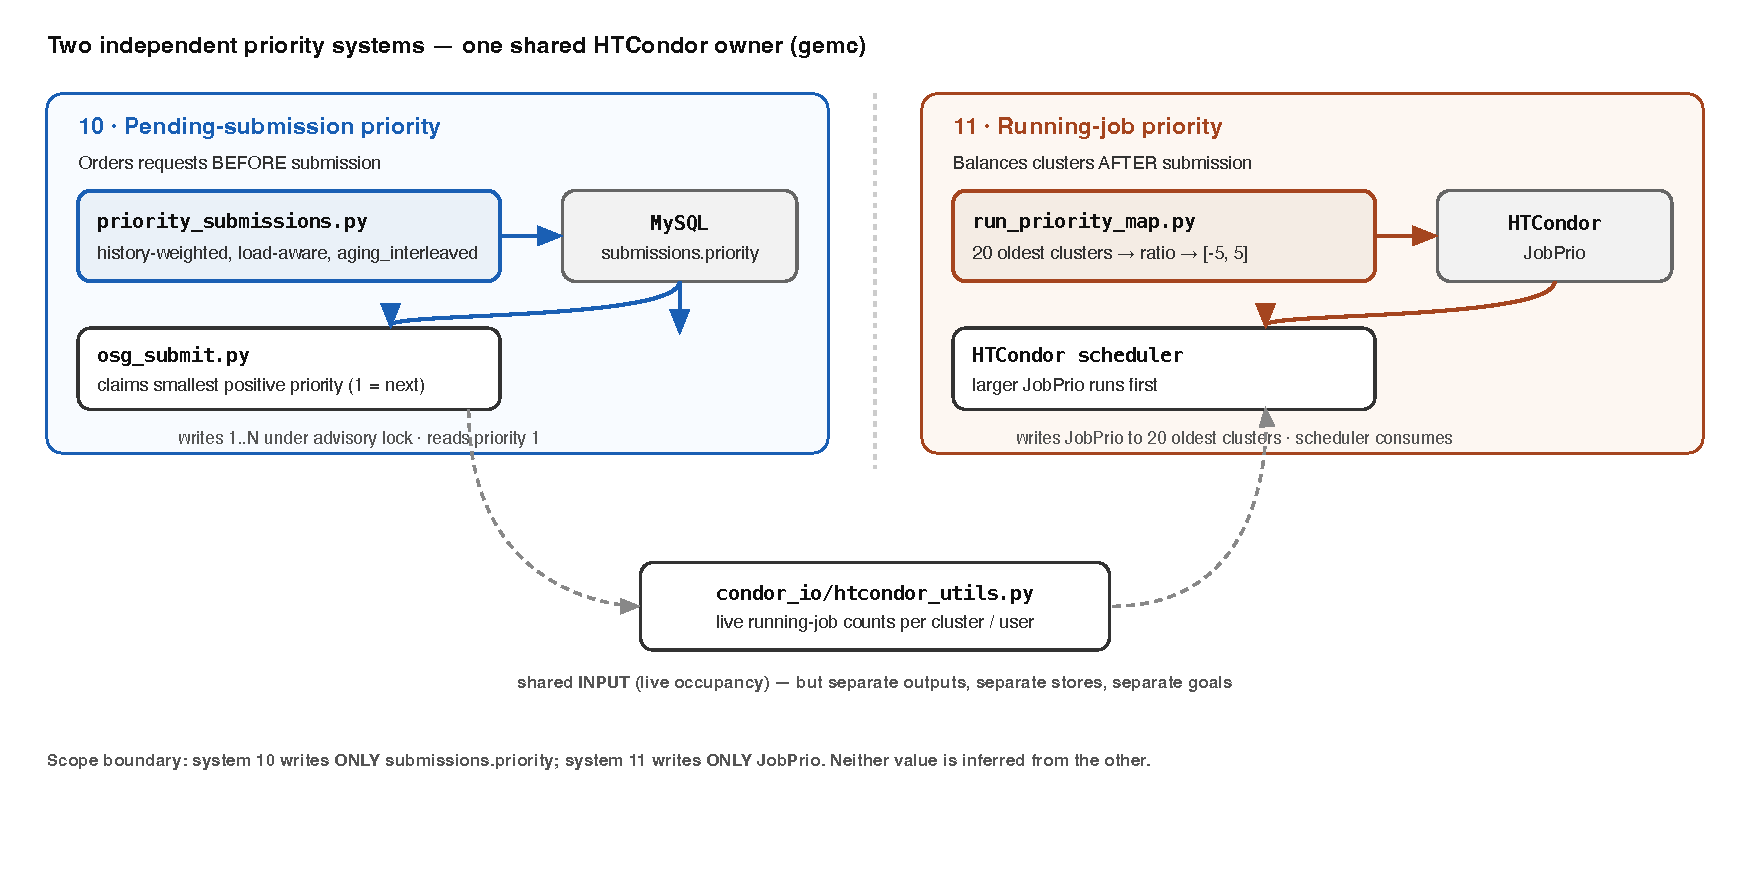
\includegraphics[width=\textwidth]{figures/fig4_two_priorities}
  \caption{The two priority systems share live-occupancy input via \texttt{htcondor\_utils.py} but are
  otherwise strictly separated --- the single most misunderstood aspect of the portal. System~10 writes only
  \texttt{submissions.priority}; system~11 writes only \texttt{JobPrio}; neither value is inferred from the
  other.}
  \label{fig:priorities}
\end{figure}

